% Options for packages loaded elsewhere
\PassOptionsToPackage{unicode}{hyperref}
\PassOptionsToPackage{hyphens}{url}
%
\documentclass[
  12pt,
]{article}
\usepackage{lmodern}
\usepackage{amssymb,amsmath}
\usepackage{ifxetex,ifluatex}
\ifnum 0\ifxetex 1\fi\ifluatex 1\fi=0 % if pdftex
  \usepackage[T1]{fontenc}
  \usepackage[utf8]{inputenc}
  \usepackage{textcomp} % provide euro and other symbols
\else % if luatex or xetex
  \usepackage{unicode-math}
  \defaultfontfeatures{Scale=MatchLowercase}
  \defaultfontfeatures[\rmfamily]{Ligatures=TeX,Scale=1}
\fi
% Use upquote if available, for straight quotes in verbatim environments
\IfFileExists{upquote.sty}{\usepackage{upquote}}{}
\IfFileExists{microtype.sty}{% use microtype if available
  \usepackage[]{microtype}
  \UseMicrotypeSet[protrusion]{basicmath} % disable protrusion for tt fonts
}{}
\makeatletter
\@ifundefined{KOMAClassName}{% if non-KOMA class
  \IfFileExists{parskip.sty}{%
    \usepackage{parskip}
  }{% else
    \setlength{\parindent}{0pt}
    \setlength{\parskip}{6pt plus 2pt minus 1pt}}
}{% if KOMA class
  \KOMAoptions{parskip=half}}
\makeatother
\usepackage{xcolor}
\IfFileExists{xurl.sty}{\usepackage{xurl}}{} % add URL line breaks if available
\IfFileExists{bookmark.sty}{\usepackage{bookmark}}{\usepackage{hyperref}}
\hypersetup{
  pdftitle={Welcome Home --- Now Vote!},
  pdfauthor={Kevin Morris},
  hidelinks,
  pdfcreator={LaTeX via pandoc}}
\urlstyle{same} % disable monospaced font for URLs
\usepackage[margin=1in]{geometry}
\usepackage{longtable,booktabs}
% Correct order of tables after \paragraph or \subparagraph
\usepackage{etoolbox}
\makeatletter
\patchcmd\longtable{\par}{\if@noskipsec\mbox{}\fi\par}{}{}
\makeatother
% Allow footnotes in longtable head/foot
\IfFileExists{footnotehyper.sty}{\usepackage{footnotehyper}}{\usepackage{footnote}}
\makesavenoteenv{longtable}
\usepackage{graphicx}
\makeatletter
\def\maxwidth{\ifdim\Gin@nat@width>\linewidth\linewidth\else\Gin@nat@width\fi}
\def\maxheight{\ifdim\Gin@nat@height>\textheight\textheight\else\Gin@nat@height\fi}
\makeatother
% Scale images if necessary, so that they will not overflow the page
% margins by default, and it is still possible to overwrite the defaults
% using explicit options in \includegraphics[width, height, ...]{}
\setkeys{Gin}{width=\maxwidth,height=\maxheight,keepaspectratio}
% Set default figure placement to htbp
\makeatletter
\def\fps@figure{htbp}
\makeatother
\setlength{\emergencystretch}{3em} % prevent overfull lines
\providecommand{\tightlist}{%
  \setlength{\itemsep}{0pt}\setlength{\parskip}{0pt}}
\setcounter{secnumdepth}{5}
\usepackage{rotating}
\newcommand{\beginsupplement}{\setcounter{table}{0}  \renewcommand{\thetable}{A\arabic{table}} \setcounter{figure}{0} \renewcommand{\thefigure}{A\arabic{figure}}}
\usepackage{setspace}
\usepackage{lineno}
\linenumbers
\usepackage{booktabs}
\usepackage{longtable}
\usepackage{array}
\usepackage{multirow}
\usepackage{wrapfig}
\usepackage{float}
\usepackage{colortbl}
\usepackage{pdflscape}
\usepackage{tabu}
\usepackage{threeparttable}
\usepackage{threeparttablex}
\usepackage[normalem]{ulem}
\usepackage{makecell}
\usepackage{xcolor}
\newlength{\cslhangindent}
\setlength{\cslhangindent}{1.5em}
\newenvironment{cslreferences}%
  {\setlength{\parindent}{0pt}%
  \everypar{\setlength{\hangindent}{\cslhangindent}}\ignorespaces}%
  {\par}

\title{Welcome Home --- Now Vote!\thanks{The author thanks Jacob Faber, Jeff Manza, Myrna Pérez, Ariel White, and Peter Miller for their comments on this project. All errors are my responsibility.}}
\usepackage{etoolbox}
\makeatletter
\providecommand{\subtitle}[1]{% add subtitle to \maketitle
  \apptocmd{\@title}{\par {\large #1 \par}}{}{}
}
\makeatother
\subtitle{Voting Rights Restoration and Post-Supervision Participation}
\author{Kevin Morris\footnote{Researcher, Brennan Center for Justice at NYU School of Law, 120 Broadway Ste 1750, New York, NY 10271 (\href{mailto:kevin.morris@nyu.edu}{\nolinkurl{kevin.morris@nyu.edu}})}}
\date{November 05, 2020}

\begin{document}
\maketitle
\begin{abstract}
Objective: Past research demonstrates that formerly incarcerated individuals turn out at very low rates. Executive Order 181 in New York State allows us to test whether restoring voting rights at an in-person meeting while an individual is still on parole can increase their post-supervision registration and turnout.

Methods: By linking administrative parole records with the registered voter file I estimate individual-level turnout. I use an interrupted time series and two-stage least squares approach to estimate the causal effect of Executive Order 181 on post-supervision participation.

Results: I find that Executive Order 181 increased post-supervision registration and turnout for individuals discharged from parole as a whole; these results, however, mask racial heterogeneity. Although the participation of non-Black individuals increased substantially, the treatment effect for Black individuals was either much smaller or nonexistent.

Conclusion: State policy can meaningfully increase the political participation of individuals even after they are no longer on parole. However, at least in the case of New York State, rights restoration prior to parole discharge appears less effective for Black individuals, who make up roughly 40 percent of the formerly incarcerated population.
\end{abstract}

\pagenumbering{gobble}
\pagebreak
\doublespacing

\pagenumbering{arabic}

\hypertarget{introduction}{%
\section*{Introduction}\label{introduction}}
\addcontentsline{toc}{section}{Introduction}

Collectively, felony disenfranchisement laws actively disenfranchise as many as 5.2 million American citizens. Of these, the majority are no longer incarcerated, but are either on parole, probation, or are disenfranchised after completing their sentence (Uggen et al. \protect\hyperlink{ref-Uggen2020}{2020}). The effects of felony disenfranchisement, however, might be even broader: there is some evidence that incarceration continues to structure political participation even after an individual is no longer legally disenfranchised. Some literature argues that interactions with the criminal justice system leaves residents less likely to vote in the future (Weaver and Lerman \protect\hyperlink{ref-Weaver2010}{2010}; White \protect\hyperlink{ref-White2019}{2019}), though other research casts some doubt on this conclusion (Gerber et al. \protect\hyperlink{ref-Gerber2017}{2017}). One thing is clear: As Burch (\protect\hyperlink{ref-Burch2011}{2011}) and others have shown, turnout rates among the formerly incarcerated are extremely low. Formal disenfranchisement policy, the literature has made clear, is just one piece of an interlocking system that serves to reduce the representation of minority and marginalized voters. The incarcerated population is drawn from a pool of individuals who rarely vote, both prior to and after their incarceration. To address only the formal laws contributing to disenfranchisement without also interrogating efforts to boost post-supervision participation risks leaving much of the system of effective disenfranchisement undisturbed. New York State offers us the opportunity to test how the timing and method of the re-instation of voting rights structures post-supervision participation.

Prior to 2018, New Yorkers convicted of felony offenses and sentenced to prison were disenfranchised until they had completed all terms of their sentence --- their period of incarceration as well as any parole term. For New Yorkers on life parole or sentenced to life in prison, this law resulted in effective lifetime disenfranchisement. New Yorkers sentenced to felony probation, on the other hand, did not lose their voting rights.

In the spring of 2018,\footnote{Although the executive order was signed on April 18th, it did not go into effect until May 18th.} Governor Andrew Cuomo signed Executive Order 181 which restored voting rights to most New Yorkers on parole. The policy change directly re-enfranchised individuals who were still on parole on election day, but the consequences might be further reaching. For instance, the change in policy is also perhaps beneficial for felony probationers: despite the fact that probationers do not formally lose their voting rights, there is evidence that confusion around the law contributes to \emph{de facto} disenfranchisement among probationers (Drucker and Barreras \protect\hyperlink{ref-Drucker2005}{2005}). By re-enfranchising anyone not actively incarcerated, the rules were substantially simplified.

The executive order may also have increased the political participation of \emph{formerly} disenfranchised individuals. Prior to the policy change, formerly incarcerated individuals had their voting rights restored automatically upon the completion of their parole term. Beginning in 2010, New York State began including information about voter eligibility in parole discharge packets, a change that Meredith and Morse (\protect\hyperlink{ref-Meredith2013}{2013}) indicates did not increase turnout. Executive Order 181 both changed the \emph{timing} of rights restoration (upon release from prison, not the end of parole) and the \emph{manner} of restoration (via an in-person meeting, rather than in a discharge packet). This study tests the bundled effect of these changes on individuals whose legal right to vote was not changed by the executive order because they were discharged from parole before the registration deadline for the 2018 midterm elections.

Shortly after the implementation of the executive order, Acting Deputy Commissioner for Community Supervision Ana Enright sent a memorandum to New York State parole officers detailing the Department of Corrections' new approach.\footnote{See \url{https://nyassembly.gov/member_files/139/webdocs/82103.pdf}.} The memorandum directs all parole officers to present individuals on parole with voter registration forms and to explain their purpose. Parole officers are instructed to offer any assistance needed, including help filling out the registration form. In addition to these directives, the memorandum communicates that voter registration is to receive ``high priority attention,'' and it separately calls the program ``a \textbf{priority} initiative'' {[}emphasis in the original{]}. Thus, the executive order demands not only that re-enfranchised individuals receive in-person notification of their voting rights, but also that parole officers prioritize their registration.

In the analysis below, I examine the effect of Executive Order 181 on individuals who finished parole before October 10th, 2018 (the registration deadline for the 2018 general election) --- in other words, voters whose legal eligibility to vote was not changed, but whose behavior may nonetheless have been impacted. By examining the effect of rights restoration in the context of a personal relationship with a parole officer against a status quo in which formerly incarcerated individuals were informed of their eligibility via brochures in a parole discharge packet, Executive Order 181 offers us the opportunity to build on existing research. Do these human interactions repair damage done to the formerly incarcerated individual's relationship to the state (Lerman and Weaver \protect\hyperlink{ref-Lerman2014}{2014})? Or do parole officers exhibit biases against their stewards, making them ineffective or uneven conduits for restoration (see, for instance, White, Nathan, and Faller \protect\hyperlink{ref-White2015}{2015})?

\hypertarget{notification-re-enfranchisement-and-turnout}{%
\section*{Notification, Re-enfranchisement, and Turnout}\label{notification-re-enfranchisement-and-turnout}}
\addcontentsline{toc}{section}{Notification, Re-enfranchisement, and Turnout}

Whether --- and to what extent --- incarceration causes lower turnout among citizens is the subject of some debate in the literature. Although Gerber et al. (\protect\hyperlink{ref-Gerber2017}{2017}) argues that prison does not materially impact post-incarceration turnout, White (\protect\hyperlink{ref-White2019}{2019}) finds that jail time can decrease the future turnout of misdemeanants. Regardless of the causal impact of incarceration on turnout, however, it is well established that formerly incarcerated individuals turn out at relatively low rates (see, for instance, Burch \protect\hyperlink{ref-Burch2011}{2011}). Thus, even if incarceration does not lead to lower turnout, policies targeting individuals caught up in the criminal justice system might still be effective at increasing their turnout, both while serving their sentence and afterwards.

Meredith and Morse (\protect\hyperlink{ref-Meredith2013}{2013}) examines the direct effect of changing rights restoration notification policies in New Mexico, New York, and North Carolina. In the case of New Mexico, formerly disenfranchised individuals began automatically receiving a certificate attesting to their eligibility to vote, a certificate they were previously required to affirmatively request. In New York and North Carolina, parole discharge packets began including explicit information about eligibility to vote. Meredith and Morse (\protect\hyperlink{ref-Meredith2013}{2013}) finds no effect on turnout from notification in the absence of eligibility changes. In the three states studied in Meredith and Morse (\protect\hyperlink{ref-Meredith2013}{2013}), however, newly re-enfranchised individuals received this information as part of a discharge packet. Moreover, in the case of New York, the brochure included in the discharge packet did not explicitly inform individuals that their voting rights had been restored. Formerly convicted individuals are very often confused about their eligibility to vote (Drucker and Barreras \protect\hyperlink{ref-Drucker2005}{2005}; Manza and Uggen \protect\hyperlink{ref-locked_out}{2008}), and it is possible that these brochures, non-explicit and bundled with other documents as they were, were ineffective at dispelling misinformation.

Meredith and Morse (\protect\hyperlink{ref-Meredith2015}{2015}) examines the impact of ending permanent disenfranchisement in Iowa. Prior to 2005 (and after 2011), individuals with felony convictions were permanently disenfranchised unless they submitted an application to the governor. Executive Order 42 eliminated this requirement, instead re-enfranchising individuals automatically upon sentence completion. Although all formerly disenfranchised individuals were re-enfranchised upon the signing of the Executive Order, not all re-enfranchised individuals were informed of their change in status. Meredith and Morse (\protect\hyperlink{ref-Meredith2015}{2015}) leverages differences in notification to test whether the notification increased turnout, finding a strong positive effect.

Gerber et al. (\protect\hyperlink{ref-Gerber2015}{2015}) built on the quasi-experimental design of Meredith and Morse (\protect\hyperlink{ref-Meredith2015}{2015}), conducting a field experiment in Connecticut in advance of the 2012 presidential election. In their field experiment, some formerly disenfranchised (but eligible) residents were reminded of their eligibility; others were not. Like Meredith and Morse (\protect\hyperlink{ref-Meredith2015}{2015}), they find evidence that these reminders successfully increased turnout. ``Whatever the participatory consequences of incarceration,'' they conclude, ``they are not in large part impossible to overcome'' (924). Even if incarceration does not decrease individuals' propensity to vote, there is reason to believe that reminding formerly incarcerated individuals of their rights increases participation.

This research provides valuable insight into mechanisms that can increase the turnout of formerly disenfranchised individuals. While information included in discharge packets seems ineffective at boosting turnout, there is some evidence that notification delivered on its own is successful. Nevertheless, the research to date has examined the effect of rights restoration notification outside a personal relationship on post-supervision turnout. An in-person meeting might be more effective at dispelling confusion about eligibility than a brochure included in a discharge packet.

There is reason to believe that some of the negative treatment effects of incarceration arise from the very nature of person-to-person relationships in the criminal justice system. Lerman and Weaver (\protect\hyperlink{ref-Lerman2014}{2014}) argues that contact with the criminal justice system can uniquely structure democratic participation more than other types of government contact. ``It may also be,'' they write, ``that social benefits {[}arising from non-criminal justice contact with the state{]} are less visible to citizens because they often occur through the mail, rather than through personal contact with government agencies or officials, making it easier to disconnect social benefits from government and the political system'' (93). Because Executive Order 181 operates \emph{not} through the mail (or discharge packet) but rather through ``personal contact with government\ldots{} officials,'' its effects may differ from the mail notification programs. The social benefits (restoration of voting rights) might be communicated more effectively and in ways that improve the formerly incarcerated individuals' opinions of their democratic state, thus increasing turnout further.

Of course, reliance on a human-mediated system to deliver social benefits poses potential practical and scientific complications. A notification sent in the mail is a binary treatment: the letter was either sent or not sent. Communicating the restoration of voting rights through human interaction means that the treatment might vary by individuals: if individuals have a warm relationship with their parole officer, they may be strongly encouraged to register and participate. On the other hand, if parole officers are biased against their charges (due either to racial hostility, personal dislike, or expected partisan affiliation) they may not provide any effective treatment at all. Thus, while the communication of voting rights restoration in the context of a personal relationship has the potential to deliver much larger benefits, it also opens the door to potential discrepancies in treatment.

I therefore expect that Executive Order 181 will increase the turnout of individuals even after they are discharged from parole through two causal mechanisms. As the previous literature has established, notification of voting rights can increase turnout, and being informed by a parole officer likely leaves a formerly paroled individual more sure of her voting rights than a brochure. Secondly, the interpersonal nature of the relationship is expected to more effectively repair (some of) the damage done to the formerly incarcerated individual's interpretation of the state. Individual, in-person invitations to rejoin the body politic are likely effective.

\hypertarget{data}{%
\section*{Data}\label{data}}
\addcontentsline{toc}{section}{Data}

\hypertarget{criminal-justice-data}{%
\subsection*{Criminal Justice Data}\label{criminal-justice-data}}
\addcontentsline{toc}{subsection}{Criminal Justice Data}

Individual-level parole records come from the New York State Department of Corrections and Community Supervision (NYSDOCCS). The data includes a host of information, including: first, middle, and last name; date of birth; class of offense; incarceration start and end dates; dates of parole; race / ethnicity; and others. This analysis is limited to individuals incarcerated for felony offenses. Individuals convicted of misdemeanors are not disenfranchised in New York State.

Following Executive Order 181, the Department of Corrections and Community Supervision began indicating on their online Parolee Lookup Tool whether an individual had her voting rights restored. By using the identification number provided from the public records request and this website, I identify individuals who had their voting rights restored.\footnote{Not all individuals listed in the public records request data are included in the lookup tool. Roughly 1 percent are not in the online lookup.} There were 3,093 individuals who were discharged from parole before the registration deadline whose rights were restored while still under supervision. Roughly 1,200 individuals who were discharged between the effective date of the executive order and the registration deadline did not have voting rights restored, due largely to their status as noncitizens.

\hypertarget{voter-file-data}{%
\subsection*{Voter File Data}\label{voter-file-data}}
\addcontentsline{toc}{subsection}{Voter File Data}

In New York, the registered voter file includes first, middle, and last name; date of birth; vote history; and other information. I use a snapshot of the registered voter file from March 3rd, 2019.

\hypertarget{matching}{%
\subsection*{Matching}\label{matching}}
\addcontentsline{toc}{subsection}{Matching}

Turnout in the 2018 midterm election is estimated by matching the parole records with the registered voter file. I match individuals in each dataset using first name, middle name, last name, and date of birth. To be considered a match, records must have the exact same birth date. The first and last names must also be exact matches (conditional on the adjustments discussed below). Middle names must match exactly as well, except for if one record has only a middle initial, which is allowed to match to a full middle name in the other set of records.

I adopt the test developed in Meredith and Morse (\protect\hyperlink{ref-Meredith2013}{2013}) to test the prevalence of false positives. I slightly alter the date of birth reported in the parole discharge dataset to create false records. Comparing the number of matches between these ``fake'' discharge records and the voter file with the number of matches between the ``true'' records and the voter file provides an estimate of how frequently false positives occur. Table \ref{tab:change-dobs} shows the results of true matches, as well as when I construct a set of fake records by adding or subtracting 35 days from an individual's birthdate. This analysis indicates that false positives account for between 0.6 and 0.7 percent of all matches, a share that is probably too small to have any material impact on the overall analysis.

\begin{singlespace}
\begin{table}[H]

\caption{\label{tab:shift-dobs-chunk}\label{tab:change-dobs} Results of Shifting Birthdates}
\centering
\begin{tabular}[t]{cc}
\toprule
Group & \makecell[l]{Number of Matches Between\\DOCCS and Voter File Records}\\
\midrule
Actual Birthdate & 69,644\\
Birthdate + 35 Days & 502\\
Birthdate - 35 Days & 426\\
\bottomrule
\end{tabular}
\end{table}
\end{singlespace}

Testing for false negatives is more challenging. If an individual marries and changes her name after being discharged from parole, for instance, I will not identify her using this matching methodology. Similarly, ``John Doe'' and ``Jonathan Doe'' would not result in a match. To reduce the likelihood of these false negatives I remove all punctuation from all names, and standardize capitalization. A record with a last name of ``O'Donnell'' in one dataset, therefore, would match a last name of ``O DONNELL'' in the other (provided the other criteria are satisfied). Such standardizations, however, will miss individuals who change their names entirely. For three reasons this is not expected to present major challenges: firstly, far more women change their last names than men, and women make up less than 10 percent of individuals who have been discharged from felony parole. Secondly, because both discharge and voter registration are legal records, individuals are likely to be recorded using their full names (that is to say, an individual is unlikely to be ``John'' in one set of records and ``Jonathan'' in the other). Finally, rates of false negatives are likely to be constant within the state during the study period, and there is no reason to believe that these false negatives would be associated with being discharged from parole after the executive order went into effect.

\hypertarget{research-design}{%
\section*{Research Design}\label{research-design}}
\addcontentsline{toc}{section}{Research Design}

I exploit randomness in discharge date from parole in New York State to determine the efficacy of the policy change, measured both using turnout in the 2018 election, and registration status as of the registration deadline for the same contest. All individuals discharged from parole after the effective date of the executive order are assigned to the treatment group; individuals discharged earlier are assigned to the control group. When we limit the pool of formerly incarcerated individuals to those discharged from parole in 2017 and 2018, the control and treatment voters look virtually identical along observable characteristics (see Table \ref{tab:demo-rd}). The assignment to treatment is as nearly random as can be hoped for in the context of a natural experiment. The basic design is therefore an interrupted time series, in which I test whether individuals discharged after the executive order took effect registered and turned out at higher rates than those discharged before the policy change. This allows me to test the intention-to-treat (ITT) effect of the executive order; in other words, the extent to which the policy change impacted overall registration and turnout among formerly incarcerated individuals.

Not all formerly incarcerated individuals were eligible to have their rights restored. Noncitizens, for instance, and individuals who were re-arrested while on parole did not have their voting rights restored. Individuals who fall into these categories and were discharged after the executive order are nonetheless included in the ITT group, even though they were not in fact treated (put differently, they did not ``comply'' with being assigned to the treatment group). Because some individuals in the ITT group went untreated, the ITT effect will be biased towards zero. The ITT therefore cannot be understood as the causal effect of rights restoration on the turnout of the individuals whose rights were actually restored.

Two-stage least squares approaches are commonly used to estimate the causal effect of treatment in a scenario with ``imperfect compliance'' (see, for instance, Ansolabehere, Iyengar, and Simon \protect\hyperlink{ref-Ansolabehere1999}{1999}; Gerber and Green \protect\hyperlink{ref-Gerber2000}{2000}; Milligan, Moretti, and Oreopoulos \protect\hyperlink{ref-Milligan2004}{2004}; Lassen \protect\hyperlink{ref-Lassen2004}{2004}; Sondheimer and Green \protect\hyperlink{ref-Sondheimer2010}{2010}). By using the random assignment to treatment as an instrument for actual treatment, the complier average causal effect (CACE) can be estimated. Here, whether someone was discharged from parole after the executive order went into effect (that is, whether someone was assigned to the treatment group) instruments whether their rights were actually restored (whether they ``complied'' with being treated). Of course, using terms like ``compliance'' here is slightly misleading: the individuals who did not ``comply'' were legally barred from having voting rights restored (or, in the case of noncitizens, conferred) --- they had little influence over whether or not they were actually treated, after being assigned to the treatment group. Nevertheless, I use this nomenclature to make the ties to existing methodological research clear.

\hypertarget{results}{%
\section*{Results}\label{results}}
\addcontentsline{toc}{section}{Results}

Before estimating the interrupted time series model, I establish that any change in turnout between those discharged before and after the policy went into effect is not due to underlying trends. It is possible, for instance, that individuals discharged from parole shortly before an election are more likely to vote irrespective of policy intervention.

Table \ref{tab:to-18-logit-short} presents an ordinary least squares regression using only the control voters. The variable \emph{Days off Parole Before Election} indicates the number of days between an individual's discharge date and the 2018 election. As the table makes clear, for individuals discharged between January 1, 2017, and May 17, 2018 --- the day before the executive order went into effect --- there was no relationship between time-off-parole and 2018 turnout and registration.

\begin{singlespace}

\input{"../../temp/table3.tex"}
\end{singlespace}

To further demonstrate the validity of the interrupted time series model, Table \ref{tab:demo-rd} shows the demographic characteristics of individuals in the control group (those discharged between January 1st, 2017, and May 17th, 2018) and the ITT group (those discharged between May 18th and October 12th, 2018) with a difference-of-means t-test. With the exception of age, the control and ITT groups are statistically indistinguishable from one another, further demonstrating the validity of the natural experiment conceptualization. The control group is, on average, slightly older, which Table \ref{tab:to-18-logit-short} indicates makes them more likely to vote and be registered. To the extent the control group perhaps has a marginally higher participation propensity than the ITT group, this setup is (slightly) biased against finding a significant increase due to the executive order.

\begin{singlespace}

\input{"../../temp/table_whatever2.tex"}
\end{singlespace}

Having established the validity of the interrupted time series model, Table \ref{tab:to-18-logit} presents the results of OLS specifications exploring whether individuals who were discharged on or after May 18th, 2018, registered and turned out at higher rates than those discharged earlier. Models 1 and 2 ask whether individuals in the treatment group were more likely to be registered prior to the registration deadline, while Models 3 and 4 test turnout in the 2018 midterm election. Models 1 and 3 estimate the overall treatment effect, while Models 2 and 4 investigate whether the treatment effect was different for Black individuals than others.

In Model 5 I estimate a ``placebo'' regression as a final check against the possibility that individuals discharged in the summer of an election year turn out at higher rates. Model 5 includes all individuals last discharged between January 1, 2015, and October 14th, 2016. The dummy \emph{Discharged After EO 181} measures whether an individual was discharged after May 18, 2016, and the dependent variable is turnout in the 2016 general election. In each model, robust standard errors are clustered by control / intention-to-treat status.

\begin{singlespace}

\input{"../../temp/table4.tex"}
\end{singlespace}

The coefficients on \emph{Discharged After EO 181} in Table \ref{tab:to-18-logit} indicate that individuals discharged after the policy changed registered and turned out at higher rates than those discharged earlier. As expected, the coefficient is nonsignificant in the placebo regression, implying that individuals discharged shortly before an election are not generally more likely to vote. Individuals discharged after the executive order went into effect were 0.8 points more likely to register (Model 1) and 0.6 percentage points more likely to vote (Model 3).

Models 2 and 4 demonstrate that there is large racial heterogeneity in these effects. The interaction effect --- \emph{Black × Discharged After EO 181} --- is negative, large relative to the general treatment effect, and statistically significant in both models. The executive order was apparently substantially more effective at boosting registration and turnout for non-Black than Black individuals.

Why would the intervention have increased turnout and registration among non-Black individuals and have had no effect on Black individuals? This difference may be explained in part through the causal mechanisms I have argued are at play in the case of Executive Order 181. As discussed above, many formerly incarcerated individuals are unsure about their legal eligibility to cast a ballot. It is possible that, prior to the policy change, formerly incarcerated Black individuals were more aware of their post-supervision voting rights. This would reduce the marginal efficacy of the information-communicating aspect of Executive Order 181.

If this were the case, we would expect to see higher turnout and registration rates for Black individuals in the control group. And, indeed, that is precisely what we observe. Table \ref{tab:re} shows that considerably more Black individuals in the control group were registered in time for and participated in the 2018 general election than other control individuals. This is in line with Meredith and Morse (\protect\hyperlink{ref-Meredith2013}{2013}) which similarly finds higher post-supervision turnout among Black individuals in New York State. Post-treatment, the gap in turnout disappears, but Black individuals discharged after the executive order went into effect were still more likely to be registered than others. Although this does not rule out other potential explanations, it is possible that the executive order did not increase the information available to Black individuals because it was information to which they would have otherwise still had access. Nevertheless, the success of Executive Order 181 is tempered by these disparate outcomes. Not only did the policy fail to boost turnout or registration for some 40 percent of the treatment group (see Table \ref{tab:demo-rd}); it was also precisely the racialized individuals who are most over-represented in the criminal justice system whose post-intervention behavior was left unchanged.

\begin{singlespace}

\input{"../../temp/table_whatever3.tex"}
\end{singlespace}

\hypertarget{sensitivity-analysis}{%
\subsection*{Sensitivity Analysis}\label{sensitivity-analysis}}
\addcontentsline{toc}{subsection}{Sensitivity Analysis}

The models in Table \ref{tab:to-18-logit} leverage a large pool of voters on either side of the effective date of the executive order; it is perhaps implausible that voters discharged in the early months of 2017 are truly good controls for those discharged in the summer of 2018, despite the above diagnostics. To explore whether these results are sensitive to the window used around the effective date, Figure \ref{fig:sens} re-estimates Models 3 and 5 in Table \ref{tab:to-18-logit} using different windows. In the most conservative window, I include only individuals discharged one month before or after the executive order went into effect (and the same period in 2016). As the window increases, we gain more observations --- and therefore statistical power --- at the cost of further temporal distance between control and ITT observations.\footnote{The post-treatment window never extends past the 2018 and 2016 registration deadlines; the estimates at the far right of Figure \ref{fig:sens}, therefore, are only extending the window backwards in time.}

\begin{figure}[H]

{\centering 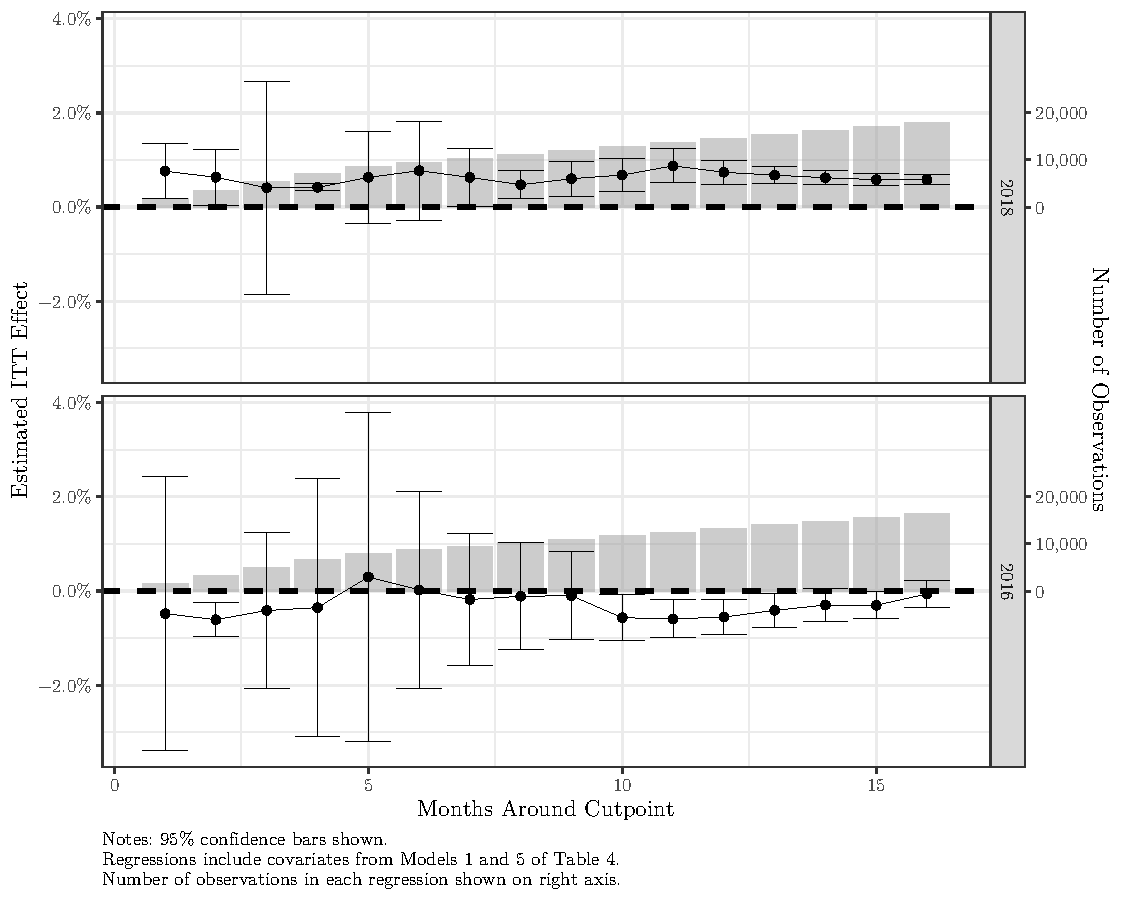
\includegraphics{table_embed_files/figure-latex/sensitivity-1} 

}

\caption{\label{fig:sens}Estimated Treatment Effect by Window Size}\label{fig:sensitivity}
\end{figure}

Although a small handful of the windows in the 2018 regressions are statistically nonsignificant, the size of the estimated treatment effect is stable and significant at the 95\% level in 13 of the 16 models. The estimated effects in the placebo regressions, on the other hand, are consistently nonsignificant (in 10 specifications) or negative (in the remaining 6 specifications). This means that voters discharged in the summer before an election are perhaps \emph{less} likely to vote absent treatment. This implies our estimated effect of the executive order is, if anything, somewhat conservative.

\hypertarget{instrumental-variables-approach}{%
\subsection*{Instrumental Variables Approach}\label{instrumental-variables-approach}}
\addcontentsline{toc}{subsection}{Instrumental Variables Approach}

The analyses in the previous sections indicate that the executive order was successful at increasing turnout and registration among formerly incarcerated individuals as a group. They do not, however, provide us an estimate of the effect of rights restoration prior to parole discharge on the specific individuals who were eligible for treatment. To answer this question, we must specifically control for whether an individual \emph{actually} had his rights restored before he was discharged from parole --- not simply whether he was discharged after the policy change. I consider individuals discharged on or after May 18 whose rights were in fact restored prior to discharge from parole as ``compliers.'' As mentioned above, some 1,200 individuals who were discharged after the policy went into effect did not have their voting rights restored.

A two-stage least squares model allows me to leverage the random assignment to treatment to identify the complier average causal effect (CACE). To use assignment to treatment as an instrument for compliance, assignment to treatment group must be uncorrelated with the outcome variable except via the treatment (Angrist, Imbens, and Rubin \protect\hyperlink{ref-Angrist1996}{1996}). In other words, we can only uncover the CACE in this setup if, in the absence of the policy change, individuals discharged from parole before and after May 18 would have registered and voted at the same rate in 2018. The nonsignificance of the coefficients \emph{Days off Parole} in Tables \ref{tab:to-18-logit-short} and \ref{tab:to-18-logit}, and the general nonsignificance of the placebo regressions in Figure \ref{fig:sens} indicate that this condition is met.

Table \ref{tab:iv-tab} presents the results of the two-stage least squares regression. Each model includes \emph{Rights Restored Before Discharge} (instrumented by \emph{Discharged After EO 181}) while Models 2 and 4 once again test whether the CACE was different for Black individuals than for non-Black individuals. \emph{Black × Rights Restored Before Discharge} is instrumented by \emph{Black × Discharged After EO 181}. As before, robust standard errors are clustered by treatment assignment group.

\begin{singlespace}

\input{"../../temp/table6.tex"}
\end{singlespace}

The two-stage least squares approach indicates that the CACE was roughly 1.1 percentage points (or 18 percent) for registration (Model 1) and 0.9 percentage points (or 39 percent) for turnout (Model 3). These models once again indicate that the treatment effect was substantially smaller, if not nonexistent, for Black individuals.

\hypertarget{discussion}{%
\subsection*{Discussion}\label{discussion}}
\addcontentsline{toc}{subsection}{Discussion}

Restoring voting rights to individuals on parole is an important step toward dismantling the disenfranchisement (both \emph{de jure} and \emph{de facto}) of communities of color disproportionately caught up in the criminal justice system. Prior to New York's Executive Order 181, individuals were required to wait until they finished their parole term to register to vote. That changed in 2018. On October 12th --- the registration deadline for the 2018 midterms --- there were 21,863 New Yorkers actively on parole whose voting rights had been restored. Without the executive order, every single one of these individuals would have been barred from participating. Though turnout among this group was low (just 832, or 3.81 percent, of these individuals successfully cast a ballot), their re-enfranchisement marks an important milestone for New York State.

As this analysis demonstrates, however, the impact of Executive Order 181 was not limited only to the individuals who would have been legally disenfranchised in its absence. In the case of New York State, rights restoration prior to discharge from parole was successful at boosting post-supervision participation rates. Overall turnout among formerly disenfranchised individuals increased by about 0.6 percentage points (or 29 percent), and individuals whose rights were restored saw turnout about 0.9 percentage points (or 39 percent) above where it would have been otherwise. Although the absolute impact of the policy change is small, it is meaningful given the low baseline turnout and registration among these individuals.

The mechanism through which the rules change increased turnout among these individuals is not clear. Weaver and Lerman (\protect\hyperlink{ref-Weaver2010}{2010}) argues that contact with the criminal justice system restructures how individuals understand their relationship with the government and sours their desire to participate. Automatic voting rights restoration upon the completion of a sentence likely does little to combat these negative perceptions of the government. On the other hand, an individual whose parole officer actively encourages them to register and participate may believe that the state is interested in their political participation. Such interactions may undo some of the negative socialization identified by Weaver and Lerman (\protect\hyperlink{ref-Weaver2010}{2010}).

It could also be a story of better information. As Meredith and Morse (\protect\hyperlink{ref-Meredith2015}{2015}) and Gerber et al. (\protect\hyperlink{ref-Gerber2015}{2015}) show, reminding formerly disenfranchised individuals of their restored voting rights can increase their participation (but see Meredith and Morse (\protect\hyperlink{ref-Meredith2013}{2013})). Research such as Manza and Uggen (\protect\hyperlink{ref-locked_out}{2008}) further demonstrates that many formerly incarcerated individuals wrongly believe that they are ineligible to participate. When an individual has her voting rights restored prior to discharge --- and when her parole officer is required to inform her of that fact --- she is far more likely to be confident in her voting eligibility. Of course, even voters in the control group were receiving notification of their eligibility upon discharge. If the full scope of the causal effect of Executive Order 181 is informational, it seems that information is communicated more effectively through in-person meetings. In reality, the executive order's success at boosting turnout and registration likely operated through multiple mechanisms.

Troublingly, the effect of pre-discharge rights restoration varies by race. As discussed in the body of this manuscript, this is possibly because one of the causal routes through which the executive order was expected to operate (namely, through improved information communication) had less purchase for Black voters, who may have already been well-informed about their rights. As Morris (\protect\hyperlink{ref-Morris2020}{2020}) demonstrates, voters lost to disenfranchisement in New York City come from predominantly Black neighborhoods. These dense communities may have been effective at communicating information about eligibility in the pre-treatment period.

Of course, I have hypothesized that the executive order would operate through two causal mechanisms: better information \emph{and} improved relationship with the government. Therefore, even if the executive order did not communicate information that Black individuals would not have learned from other sources, the pre-discharge restoration of voting rights should have increased their participation via a different avenue. That their participation was unaffected joins other research indicating that incarceration differentially structures turnout for Black and non-Black individuals. White (\protect\hyperlink{ref-White2019}{2019}), for instance, shows that incarceration reduces turnout more for Black voters, and Walker (\protect\hyperlink{ref-Walker2020a}{2020}) argues that Black individuals understand criminal justice involvement from a systemic --- and not individualistic --- perspective. If incarceration does more harm to Black individuals' relationship with the state, recouping their turnout may demand more than an in-person meeting to restore voting rights.

Re-enfranchising voters while they are still under formal supervision is obviously beneficial to the individuals who are on parole on election day; such policies allow them to make their voices heard. The case of Executive Order 181 also indicates that restoring voting rights prior to parole discharge has further benefits. In 2018, it increased turnout among individuals who were formally discharged from parole prior to the registration deadline, and therefore would have been eligible to vote even if their rights were not restored until the completion of their sentence. This is encouraging, demonstrating that the state has a unique opportunity to shape the future participation of individuals who are currently under their supervision. By restoring voting rights before individuals have completed their sentence, and by requiring parole officers to inform individuals of their voting rights, the state can increase the political participation of a group of often-marginalized individuals, thereby increasing the democratic representation of our elections. Nevertheless, the success of the executive order is tempered by its racially disparate effects.

\newpage

\hypertarget{references}{%
\section*{References}\label{references}}
\addcontentsline{toc}{section}{References}

\hypertarget{refs}{}
\begin{cslreferences}
\leavevmode\hypertarget{ref-Angrist1996}{}%
Angrist, Joshua D., Guido W. Imbens, and Donald B. Rubin. 1996. ``Identification of Causal Effects Using Instrumental Variables.'' \emph{Journal of the American Statistical Association} 91 (434): 444--55. \url{https://doi.org/10.1080/01621459.1996.10476902}.

\leavevmode\hypertarget{ref-Ansolabehere1999}{}%
Ansolabehere, Stephen D., Shanto Iyengar, and Adam Simon. 1999. ``Replicating Experiments Using Aggregate and Survey Data: The Case of Negative Advertising and Turnout.'' \emph{American Political Science Review} 93 (4): 901--9. \url{https://doi.org/10.2307/2586120}.

\leavevmode\hypertarget{ref-Burch2011}{}%
Burch, Traci. 2011. ``Turnout and Party Registration Among Criminal Offenders in the 2008 General Election.'' \emph{Law \& Society Review} 45 (3): 699--730. \url{https://doi.org/10.1111/j.1540-5893.2011.00448.x}.

\leavevmode\hypertarget{ref-Drucker2005}{}%
Drucker, Ernest, and Ricardo Barreras. 2005. ``Studies of Voting Behavior and Felony Disenfranchisement Among Individuals in the Criminal Justice System in New York, Connecticut, and Ohio.'' Research report. The Sentencing Project. \url{https://www.prisonpolicy.\%20org/scans/sp/fd_studiesvotingbehavior.pdf}.

\leavevmode\hypertarget{ref-Gerber2000}{}%
Gerber, Alan S., and Donald P. Green. 2000. ``The Effects of Canvassing, Telephone Calls, and Direct Mail on Voter Turnout: A Field Experiment.'' \emph{American Political Science Review} 94 (3): 653--63. \url{https://doi.org/10.2307/2585837}.

\leavevmode\hypertarget{ref-Gerber2015}{}%
Gerber, Alan S., Gregory A. Huber, Marc Meredith, Daniel R. Biggers, and David J. Hendry. 2015. ``Can Incarcerated Felons Be (Re)Integrated into the Political System? Results from a Field Experiment.'' \emph{American Journal of Political Science} 59 (4): 912--26. \url{https://doi.org/10.1111/ajps.12166}.

\leavevmode\hypertarget{ref-Gerber2017}{}%
---------. 2017. ``Does Incarceration Reduce Voting? Evidence About the Political Consequences of Spending Time in Prison.'' \emph{The Journal of Politics} 79 (4): 1130--46. \url{https://doi.org/10.1086/692670}.

\leavevmode\hypertarget{ref-Lassen2004}{}%
Lassen, David Dreyer. 2004. ``The Effect of Information on Voter Turnout: Evidence from a Natural Experiment.'' SSRN Scholarly Paper ID 475821. Rochester, NY: Social Science Research Network. \url{https://papers.ssrn.com/abstract=475821}.

\leavevmode\hypertarget{ref-Lerman2014}{}%
Lerman, Amy E., and Vesla M. Weaver. 2014. \emph{Arresting Citizenship: The Democratic Consequences of American Crime Control}. Chicago Studies in American Politics. Chicago ; London: The University of Chicago Press.

\leavevmode\hypertarget{ref-locked_out}{}%
Manza, Jeff, and Christopher Uggen. 2008. \emph{Locked Out: Felon Disenfranchisement and American Democracy}. Studies in Crime and Public Policy. New York: Oxford University Press.

\leavevmode\hypertarget{ref-Meredith2013}{}%
Meredith, Marc, and Michael Morse. 2013. ``Do Voting Rights Notification Laws Increase Ex-Felon Turnout?:'' \emph{The ANNALS of the American Academy of Political and Social Science}, November. \url{https://doi.org/10.1177/0002716213502931}.

\leavevmode\hypertarget{ref-Meredith2015}{}%
---------. 2015. ``The Politics of the Restoration of Ex-Felon Voting Rights: The Case of Iowa.'' \emph{Quarterly Journal of Political Science} 10 (1): 41--100. \url{https://doi.org/10.1561/100.00013026}.

\leavevmode\hypertarget{ref-Milligan2004}{}%
Milligan, Kevin, Enrico Moretti, and Philip Oreopoulos. 2004. ``Does Education Improve Citizenship? Evidence from the United States and the United Kingdom.'' \emph{Journal of Public Economics} 88 (9): 1667--95. \url{https://doi.org/10.1016/j.jpubeco.2003.10.005}.

\leavevmode\hypertarget{ref-Morris2020}{}%
Morris, Kevin. 2020. ``Neighborhoods and Felony Disenfranchisement: The Case of New York City.'' \emph{Urban Affairs Review}, May, 1078087420921522. \url{https://doi.org/10.1177/1078087420921522}.

\leavevmode\hypertarget{ref-Sondheimer2010}{}%
Sondheimer, Rachel Milstein, and Donald P. Green. 2010. ``Using Experiments to Estimate the Effects of Education on Voter Turnout.'' \emph{American Journal of Political Science} 54 (1): 174--89. \url{https://doi.org/10.1111/j.1540-5907.2009.00425.x}.

\leavevmode\hypertarget{ref-Uggen2020}{}%
Uggen, Christopher, Ryan Larson, Sarah Shannon, and Arleth Pulido-Nava. 2020. ``Locked Out 2020: Estimates of People Denied Voting Rights Due to a Felony Conviction.'' Research report. The Sentencing Project. \url{https://www.sentencingproject.org/wp-content/uploads/2020/10/Locked-Out-2020.pdf}.

\leavevmode\hypertarget{ref-Walker2020a}{}%
Walker, Hannah L. 2020. \emph{Mobilized by Injustice: Criminal Justice Contact, Political Participation, and Race}. 1st ed. Oxford University Press. \url{https://doi.org/10.1093/oso/9780190940645.001.0001}.

\leavevmode\hypertarget{ref-Weaver2010}{}%
Weaver, Vesla M., and Amy E. Lerman. 2010. ``Political Consequences of the Carceral State.'' \emph{American Political Science Review} 104 (4): 817--33. \url{https://doi.org/10.1017/S0003055410000456}.

\leavevmode\hypertarget{ref-White2019}{}%
White, Ariel. 2019. ``Misdemeanor Disenfranchisement? The Demobilizing Effects of Brief Jail Spells on Potential Voters.'' \emph{American Political Science Review} 113 (2): 311--24. \url{https://doi.org/10.1017/S000305541800093X}.

\leavevmode\hypertarget{ref-White2015}{}%
White, Ariel R., Noah L. Nathan, and Julie K. Faller. 2015. ``What Do I Need to Vote? Bureaucratic Discretion and Discrimination by Local Election Officials.'' \emph{American Political Science Review} 109 (1): 129--42. \url{https://doi.org/10.1017/S0003055414000562}.
\end{cslreferences}

\end{document}
